\hypertarget{cv:gestionarAtributos}{\section{Gestionar Atributos}} \label{sec:GestionarAtributos}

	Esta funcionalidad le permitirá las acciones necesarias para controlar los atributos perteneciente a una entidad y visualizarlos en una tabla en el proyecto sobre el que se está operando y solicitar el registro de uno nuevo. Para entrar a esta gestión es necesario que al menos existe una entidad dentro del proyecto.

		\subsection{Procedimiento}

			%Pasos de procedimiento
			\begin{enumerate}
				
			\item Ingrese a un proyecto existente desde la pantalla \ref{fig:GestionarProyectosColaborador}.
	
			\item Seleccione la opción \textbf{Entidades} del menú \ref{fig:MN-LPC}.
			
			\item Oprima el botón \IUAtributos{} de algún registro existente de la pantalla \ref{fig:GestionarEntidades} ''Gestionar Entidades''.
	
			\item Se mostrará la pantalla \ref{fig:GestionarAtributos} ''Gestionar Atributos''.

			%Pantalla
			\begin{figure}[h!]
				\begin{center}
					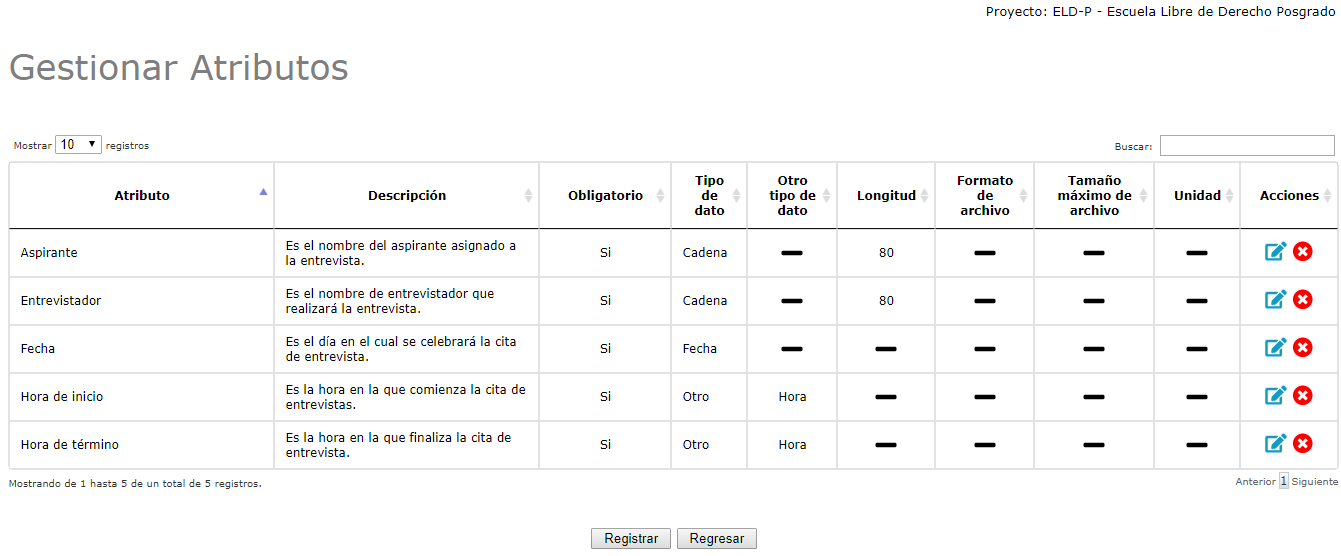
\includegraphics[scale=0.5]{roles/lider/entidades/atributos/pantallas/IU12-1-1-1gestionarAtributos}
					\caption{Gestionar Atributos}
					\label{fig:GestionarAtributos}
				\end{center}
			\end{figure}
		
				\item Seleccione la operación que desea realizar:
			
			Para (\hyperlink{cv:registrarAtributo}{Registrar}) dé clic en el botón \IURegistrar.
			
			Para (\hyperlink{cv:modificarAtributo}{Modificar}) dé clic en el icono \IUEditar{} de algún atributo ya registrado.
			
			Para (\hyperlink{cv:eliminarAtributo}{Eliminar}) dé clic en el icono \IUBotonEliminar{} de algún atributo ya registrado.
			\end{enumerate}